% !TeX spellcheck = it_IT
\documentclass[a4paper]{article}
\usepackage{amsmath}
\usepackage{pgfplots}
\usepackage{blindtext}
\usepackage[italian]{babel}
\usepackage[11pt]{moresize}
\title{\fontsize{50}{60}\selectfont FONDAMENTI DI MATEMATICA}
\author{\\\\Enrico Martini}
\date{\small versione 1.0 \\| \\2015 - 2019}


\begin{document}
	
	\maketitle
	\thispagestyle{empty}
	\newpage
	\tableofcontents
	\thispagestyle{empty}
	\newpage
	
	\section{Geometria analitica}
	\subsection{Punto}
	Rappresentazione:
	\begin{align*}
		P(x_P;y_P)
	\end{align*}
	Distanza tra due punti:
	\begin{align*}
		d = \sqrt{(x_B -x _A)^2+(y_B - y_A)^2}
	\end{align*}
	Punto medio:
	\begin{align*}
		M \left( \frac{x_A + x_B}{2} ; \frac{y_A + y_B}{2} \right)
	\end{align*}
	Baricentro:
	\begin{align*}
		G \left( \frac{x_A + x_B + x_C}{3} ; \frac{y_A + y_B + y_C}{3} \right) 
	\end{align*}
	Area di un triangolo:
	\begin{align*}
		A = \frac{1}{2} \cdot \left| \begin{array}{cc}
		x_C-x_A & y_C-y_A \\ 
		x_B-x_A & y_B-y_A
		\end{array} \right|
	\end{align*}
	
	\subsection{Retta}
	Rappresentazione:
	\begin{align*}
		y &= mx + q		&\vee&&		ax + by + c & = 0
	\end{align*}
	Retta passante per due punti:
	\begin{align*}
		\frac{y-y_A}{y_B-y_A} = \frac{x-x_A}{x_B-x_A}
	\end{align*}
	Fascio di rette passante per un punto:
	\begin{align*}
		y-y_0 = m(x-x_0)
	\end{align*}
	Distanza punto-retta:
	\begin{align*}
		d = \frac{|ax_0+by_0+c|}{\sqrt{a^2+b^2}}
	\end{align*}
		
	\subsection{Circonferenza}
	Rappresentazione:
	\begin{align*}
		x^2+y^2+ax+by+c&=0	& (x-\alpha)^2 + (y-\beta)^2 &= r^2
	\end{align*}
	Coordinate del centro:
	\begin{align*}
		C \left( -\frac{a}{2} ; -\frac{b}{2} \right)
	\end{align*}
	Raggio:
	\begin{align*}
		r = \frac{1}{2}\sqrt{a^2+b^2-4c}
	\end{align*}
	
	\subsection{Parabola}
	Rappresentazione:
	\begin{align*}
		y &= ax^2 + bx + c		&		x &= ay^2 + by + c
	\end{align*}
	Vertice:
	\begin{align*}
		V& \left(-\frac{b}{2a};-\frac{\varDelta}{4a}\right)		&		V & \left( -\frac{\varDelta}{4a} ; -\frac{b}{2a} \right) 
	\end{align*}
	
	\subsection{Ellisse}
	Rappresentazione:
	\begin{align*}
		\frac{x^2}{a^2} + \frac{y^2}{b^2} = 1
	\end{align*}
	Con $a>b$:
	\begin{align*}
		F&(\pm c ; 0)		&		c = \sqrt{a^2-b^2}
	\end{align*}
	Con $a < b$:
	\begin{align*}
		F&(0 ; \pm c)		&		c = \sqrt{b^2-a^2}
	\end{align*}
	
	\subsection{Iperbole}
	Rappresentazione:
	\begin{align*}
	\frac{x^2}{a^2} - \frac{y^2}{b^2} = 1
	\end{align*}
	Se rivolta all'asse $x$:
	\begin{align*}
		F&(\pm c ; 0)		&		c^2 &= a^2 + b^2		&		y &= \pm \frac{b}{a}x
	\end{align*}
	Se equilatera:
	\begin{align*}
		x^2 - y^2 &= a^2		&		y &= \pm x
	\end{align*}
	
	\subsubsection{Funzione omografica}
	Rappresentazione:
	\begin{align*}
	y &= \frac{ax + b}{cx + d}		&		C&\left( -\frac{d}{c} ; \frac{a}{c} \right)
	\end{align*}
	
	\subsection{Coniche generali}
	\begin{align*}
		ax^2+bxy+cy^2+dx+ey+f=0
	\end{align*}
	
	
	
	\newpage	
	\section{Trasformazioni geometriche}
	\subsubsection{Simmetria}
	 Simmetria rispetto ad un punto $P(\alpha , \beta)$ :
	 \begin{align*}
	 	\begin{cases}
	 	x' = 2 \alpha - x \\
	 	y' = 2 \beta -y 
	 	\end{cases}
	 \end{align*}
	 Simmetria rispetto all'asse $y$:
	 \begin{align*}
	 	\begin{cases}
	 	x' = -x\\
	 	y' = y
	 	\end{cases}
	 \end{align*}
	Simmetria rispetto all'asse $x$:
	\begin{align*}
		\begin{cases}
			x' = x\\
			y' = -y
		\end{cases}
	\end{align*}
	
	\subsubsection{Traslazione}
	Traslazione rispetto ad un vettore $\vec{v} (a;b)$:
	\begin{align*}
		\begin{cases}
			x'=x+a\\
			y'=y+b
		\end{cases}
	\end{align*}
	
	\subsubsection{Rotazione}
	Rotazione rispetto ad un angolo $\alpha$:
	\begin{align*}
		\begin{cases}
			x=x' \cdot \cos (\alpha) + y' \cdot \sin(\alpha)\\
			y= -x' \cdot \sin (\alpha) + y' \cdot \cos(\alpha)
		\end{cases}&
		\begin{cases}
			x'= x \cdot \cos (\alpha) - y \cdot \sin(\alpha)\\
			y'= x \cdot \sin (\alpha) + y \cdot \cos(\alpha)
		\end{cases}
	\end{align*}
	\subsubsection{Omotetia}
	Omotetia di centro $O(0;0)$ e rapporto $h$:
		\begin{align*}
	\begin{cases}
	x' = hx - x_c\\
	y' = hx - y_c
	\end{cases}
	\end{align*}
	\subsubsection{Affinità}
	\begin{align*}
		&\begin{cases}
			x'=ax+by+h\\
			y'=cx+dy+k
		\end{cases}&
		con &\varDelta = \left| \begin{matrix}
		a & b \\ 
		c & d
		\end{matrix}
		\right|\neq 0
	\end{align*}
	
	\newpage
	\section{Solidi}
	\subsubsection{Cilindro}
	\begin{align*}
		S_L & = 2p \cdot h & S_{TOT} & = S_L + 2S_B  \\
		S_B & = \pi r^2    & V       & = S_b \cdot h
	\end{align*}
	\\
	\subsubsection{Cono}
	\begin{align*}
		S_L & = \pi r a & S_{TOT} & = S_L + 2S_B            \\
		S_B & = \pi r^2 & V       & = \frac{1}{3} \pi r^2 h
	\end{align*}
	\\
	\subsubsection{Sfera}
	\begin{align*}
		S &= 4\pi r^2 & V &= \frac{4}{3} \pi r^3
	\end{align*}
	\\
	\subsubsection{Prisma}
	\begin{align*}
		S_L &= 2p \cdot h	&	S_{TOT} &= S_L +2S_B
		&			V &= S_b \cdot h
	\end{align*}
	\\
	\subsubsection{Piramide}
	\begin{align*}
		S_L &= pa	&	S_{TOT} &= S_L + S_B\\
		S_B &= l^2	&	V &= \frac{1}{3} S_B \cdot h
	\end{align*}
	
	\newpage
	\section{Geometria analitica dello spazio}

	\subsubsection{Equazione del piano}
	\begin{align*}
		\alpha : ax +by +cz+ d &= 0			&			d &= -a^2-b^2-c^2
	\end{align*}

	\subsubsection{Punto medio}
	\begin{align*}
		M \left( \frac{x_A + x_B}{2} ; \frac{y_A + y_B}{2} ; \frac{z_A + z_B}{2} \right)
	\end{align*}

	\subsubsection{Equazione di una retta}
	\begin{align*}
		\begin{cases}
		ax+by+cz+d=0\\
		ex+fy+gz+h=0
		\end{cases}
	\end{align*}

	\subsubsection{Retta passante per due punti}
	\begin{align*}
		\frac{x - x_A}{x_B - x_A} = \frac{y - y_A}{y_B - y_A} = \frac{z - z_A}{z_B - z_A} = \lambda
	\end{align*}

	\subsubsection{Distanza tra piano e punto}
	\begin{align*}
		d(A ; \alpha) = \frac{|ax_A + by_A + cz_A + d|}{\sqrt{a^2+b^2+c^2}}
	\end{align*}
	
	\subsubsection{Piano parallelo ad un altro piano passante per un punto}
	
	\begin{align*}
	\alpha = \left|
		\begin{array}{ccc}
			a & b & c \\ 
			a' & b' & c' \\ 
			a'' & b'' & c''
		\end{array}
		\right| = 0 
	\end{align*}
		
	\subsubsection{Retta perpendicolare ad un piano passante per un punto}
	
	\begin{align*}
		\frac{x-x_0}{a} = \frac{y-y_0}{b} = \frac{z-z_0}{c}
	\end{align*}
	
	\subsubsection{Piano passante per un punto perpendicolare ad una retta}
	
	\begin{align*}
		\alpha = l(x-x_0)+m(y-y_0)+n(z-z_0)=0
	\end{align*}
	
	\subsubsection{Parallelismo tra piani}
	\begin{align*}
		\frac{a}{a'} = \frac{b}{b'} = \frac{c}{c'} \ne \frac{d}{d'}
	\end{align*}
	
	\subsubsection{Perpendicolarità tra piani}
	\begin{align*}
		aa'+bb'+cc'=0
	\end{align*}
	
	\newpage
	\subsection{Calcolare i punti stazionari}
	Punti chiave:
	\begin{enumerate}
		\item Calcolare le derivate parziali del primo ordine
			\begin{align*}
				f'_x&(x,y)	&	f'_y&(x,y)
			\end{align*}
		\item Risolvere i sistema con le derivate uguali a zero
			\begin{align*}
				\begin{cases}
				f'_x(x,y)=0\\
				f'_y(x,y)=0
				\end{cases}
			\end{align*}
		\item Ricavare i punti stazionari
			\begin{align*}
				P(x_P,y_P)
			\end{align*}
		\item Calcolare le derivate parziali del secondo ordine
			\begin{align*}
				f''_{xx}&(x,y)	&	f''_{xy}&(x,y)	&	f''_{yx}&(x,y)	&	f''_{yy}&(x,y)
			\end{align*}
		\item Costruire la matrice Hessiana
			\begin{align*}
				H_f(x,y) = \left[
				\begin{array}{cc}
				f''_{xx}(x,y) & f''_{xy}(x,y) \\ 
				f''_{yx}(x,y) & f''_{yy}(x,y)
				\end{array} \right]
			\end{align*}
		\item Calcolare il determinante della matrice Hessiana
			\begin{align*}
				det(H_f(x,y)) = \left|
				\begin{array}{cc}
				f''_{xx}(x,y) & f''_{xy}(x,y) \\ 
				f''_{yx}(x,y) & f''_{yy}(x,y)
				\end{array} \right|
				\end{align*}
			\end{enumerate}
		Considerare i casi:\\
			\begin{itemize}
				\item $f''_{xx}(x_0,y_0) > 0 \wedge det(H_f) > 0 \to $ minimo locale
				\item $f''_{xx}(x_0,y_0) < 0 \wedge det(H_f) > 0 \to $ massimo locale
				\item $det(H_f) < 0 \to $ punto di sella
			\end{itemize}
			\newpage
	\subsection{Calcolare il massimo/minimo locale vincolato}		
	Punti chiave:
	\begin{enumerate}
		\item Definire la funzione lagrangiana:
			\begin{align*}
				\mathcal{L} = f(x,y) - \lambda g(x,y)
			\end{align*}
		\item Risolvere il sistema:
		\begin{align*}
			\begin{cases}
				\mathcal{L}'_x = 0\\
				\mathcal{L}'_y = 0\\
				g(x,y) = 0
			\end{cases}
		\end{align*}
		\item Calcolare le derivate parziali del secondo ordine
			\begin{align*}
			\mathcal{L}''_{xx}&(x,y)	&	\mathcal{L}''_{xy}&(x,y)	&	\mathcal{L}''_{yx}&(x,y)	&	\mathcal{L}''_{yy}&(x,y)
			\end{align*}
		\item Calcolare il determinante della matrice hessiana orlata:
		\begin{align*}
			det(\bar{H}) = \left|
			\begin{array}{ccc}
			0 & g'_x & g'_y \\ 
			g'_x & \mathcal{L}''_{xx} & \mathcal{L}''_{xy} \\ 
			g'_y & \mathcal{L}''_{yx} & \mathcal{L}''_{yy}
			\end{array} \right|
		\end{align*}
		\end{enumerate}		
		Considerare i casi:
		\begin{itemize}
			\item $det(\bar{H}) > 0 \to$ Massimo locale vincolato
			\item $det (\bar{H}) < 0 \to$ Minimo locale vincolato
			\item $det (\bar{H}) = 0 \to$ Indeterminato
		\end{itemize}

		\subsection{Calcolare il massimo/minimo globale}			
		Passi chiave:\\
		\begin{enumerate}
			\item Verificare che l'insieme sia compatto
			\item Trovare i punti stazionari interni con le derivate parziali
			\item Trovare i punti di frontiera stazionari con Lagrange
			\item Sostituire massimo/minimo per trovare i punti globali
		\end{enumerate}
			
			\newpage
	\subsection{Coordinate}
	\subsubsection{Coordinate sferiche}
	Si noti che $\rho \ge 0$, $\varphi \in [0,\pi]$ e $\varTheta \in [0,2\pi]$.
	\begin{align*}
		&\begin{cases}
			x = \rho \cdot \sin(\varphi)\cos(\varTheta)\\
			y = \rho \cdot \sin(\varphi)\sin(\varTheta)\\
			z = p \cdot \cos(\varphi)
		\end{cases}	&	p &= \sqrt{x^2+y^2+z^2}
	\end{align*}
	\begin{align*}
				\int \int \int_{D}f(x,y,z)dxdydz = \int \int \int_D f(\rho,\varphi,\varTheta) \cdot \rho^2 \cdot \sin(\varphi) d\rho d\varphi d\varTheta
	\end{align*}
	\subsubsection{Coordinate cilindriche}
	Si noti che $p \ge 0$ , $z \in \mathcal{R}$ e $\varTheta \in [0,2\pi]$.
	\begin{align*}
		&\begin{cases}
		x = \rho \cdot \cos(\varTheta)\\
		y = \rho \cdot \sin(\varTheta)\\
		z=z
		\end{cases}	&	p &= \sqrt{x^2+y^2}
	\end{align*}
	
	\subsection{Parametrizzazione}
	\subsubsection{Parametrizzazione di un ellisse}
	\begin{align*}
		&\gamma: [0,2\pi] \to \mathcal{R}^2	&	&t\to (x_c + a \cos t ; y_c + b \sin t)	&	&
		\begin{cases}
		x = a\cos t + x_c\\
		y = b \sin t + y_c
		\end{cases}
	\end{align*}
	\subsubsection{Retta tangente alla curva}
	\begin{align*}
		&\gamma: I \subseteq \mathcal{R} \to \mathcal{R}^n	&	&r: \mathcal{R} \to \mathcal{R}^n\\
		&t \to \gamma (t) = (\gamma_1 (t),\gamma_2 (t),...,\gamma_n (t))	&	&t \to \gamma (t_0) + t\gamma' (t_0) = P + t\gamma' (t_0)
	\end{align*}
	\subsubsection{Lunghezza di una curva}
	Sia $\gamma : [a,b] \to \mathcal{R}^n$ una curva regolare. Allora la lunghezza $l(\gamma)$ di $\gamma$ è finita e vale:
	\begin{align*}
		l(\gamma) = \int_{a}^{b} || \gamma'(t) ||dt
	\end{align*}
	
	\newpage
	\section{Probabilità}
	\begin{align*}
		p(E) & = \frac{casi_{POSSIBILI}}{casi_{TOTALI}} & 0 & \le p(E) \le 1
	\end{align*}
	
	\subsubsection{Probabilità della somma logica di eventi}
	\begin{align*}
		p(E_1 \cup E_2) = p(E_1) + p(E_2) - p(E_1 \cap E_2)
	\end{align*}
	
	\subsubsection{Probabilità condizionata}
	La probabilità condizionata di un evento A rispetto a un evento B è la probabilità che si verifichi A, sapendo che B è verificato.
	\begin{align*}
		p(E_1 | E_2) = \frac{p(E_1 \cap E_2)}{p(E_2)}
	\end{align*}
	
	\subsubsection{Probabilità del prodotto logico di eventi}
	\begin{align*}
		\begin{cases}
		p(E_1 \cap E_2) = p(E_1) \cdot p(E_1 | E_2)	& dipendenti\\
		p(E_1 \cap E_2) = p(E_1) \cdot p(E_2)		& indipendenti
		\end{cases}
	\end{align*}
	
	\subsubsection{Problema delle prove ripetute}
	\begin{itemize}
		\item n : numero di estrazioni
		\item k : numero delle volte in cui deve uscire
		\item p : probabilità che si verifichi
		\item q : probabilità che non si verifichi
	\end{itemize}

	\begin{align*}
		P_{k,n} = {{n}\choose{k}} p^kq^{n-k}
	\end{align*}
	
	\subsubsection{Teorema di Bayes}
	Considerando un insieme di alternative $A_{1}, ,A_{n}$ che partizionano lo spazio degli eventi $\Omega$ (ossia $A_{i} \cap A_{j} = \emptyset , \forall i\neq j$ e $\cup _{{i=1}}^{n}A_{i}=\Omega )$ si trova la seguente espressione per la probabilità condizionata:
	\begin{align*}
		p(E_i|E)= \frac{p(E_i) \cdot p(E | E_i)}{p(E)}
	\end{align*}
	
	\newpage
	\section{Calcolo combinatorio}
	\subsubsection{Disposizione semplice}
	Tutti i gruppi con $k$ elementi su $h$ elementi diversi per contenuto e ordine non ripetuti.
	\begin{align*}
		D_{n,k} = n(n-1)(n-2)...(n-k+1)
	\end{align*}

	\subsubsection{Disposizione con ripetizione}
	Numeri di k-uple ordinate $D_{n,k}$ che posso formare con n oggetti, considerando che tali oggetti possono anche essere ripetuti.
	\begin{align*}
		D'_{n,k} = n^k
	\end{align*}

	\subsubsection{Permutazione semplice}
	Tutti i gruppi con $n$ elementi con ordine diverso.
	\begin{align*}
		P_n = n! 
	\end{align*}
	
	\subsubsection{Permutazione con ripetizione}
	\begin{align*}
		P_n^{(n;k)}=\frac{n!}{n!k!}
	\end{align*}
	
	\subsubsection{Combinazione semplice}
	Scegliere $k$ elementi su $n$, senza ripetizione e senza cambiare l'ordine.
	\begin{align*}
		C_{n,k} = {{n}\choose{k}} = \frac{D_{n,k}}{P_k} = \frac{n(n-1)(n-2)...(n-k+1)}{k!} 
	\end{align*}
	
	\subsubsection{Combinazione con ripetizione}
	Si consideri un insieme I costituito da n oggetti distinti e sia k un numero naturale senza alcuna limitazione superiore.
	
	Si chiama combinazione con ripetizioni di classe k un raggruppamento non ordinato di k degli n elementi di I nel quale si possono avere ripetizioni di uno stesso elemento.\\
	\begin{align*}
		C'_{n,k} = C_{n+k-1 , k} = {{n+k-1}\choose{k}}
	\end{align*}
	
	\newpage
	\section{Goniometria}
		
	Formula fondamentale:
	\begin{align*}
	\sin ^2 (\alpha) + \cos^2 (\alpha) = 1
	\end{align*}
	Formule derivate:
	\begin{align*}
	\tan (\alpha) & = \frac{\sin (\alpha)}{\cos (\alpha)} & \cot (\alpha) & = \frac{\cos (\alpha)}{\sin (\alpha)} \\
	\sec (\alpha) & = \frac{1}{\sin (\alpha)}             & \csc (\alpha) & = \frac{1}{\cos (\alpha)}
	\end{align*}
	Somma e differenza:
	\begin{align*}
	\sin (\alpha + \beta) & = \sin (\alpha) \cdot \cos (\beta) + \cos (\alpha) \cdot \sin (\beta)\\
	\cos (\alpha + \beta) & = \cos (\alpha) \cdot \cos (\beta) - \sin (\alpha) \cdot \sin (\beta)\\
	\sin (\alpha - \beta) & = \sin (\alpha) \cdot \cos (\beta) - \cos (\alpha) \cdot \sin (\beta)\\
	\cos (\alpha - \beta) & = \cos (\alpha) \cdot \cos (\beta) + \sin (\alpha) \cdot \sin (\beta)
	\end{align*}
	Duplicazione:
	\begin{align*}
	\sin (2 \alpha) & = 2 \sin (\alpha) \cdot \cos (\alpha)	&	\cos (2 \alpha) & = \cos^2 (\alpha) - \sin^2 (\alpha)
	\end{align*}
	Bisezione:
	\begin{align*}
	\cos \left(\frac{\alpha}{2}\right) &= \pm \sqrt{\frac{1 + \cos (\alpha)}{2}} & \sin \left(\frac{\alpha}{2}\right) &= \pm \sqrt{\frac{1 - \cos (\alpha)}{2}}\\
	\tan \left(\frac{\alpha}{2}\right) &= \pm \sqrt{\frac{1-\cos (\alpha)}{1+\cos (\alpha)}} = &\frac{\sin (\alpha)}{1+\cos (\alpha)} &= \frac{1-\cos (\alpha)}{\sin (\alpha)}
	\end{align*}
	Formule parametriche:
	\begin{align*}
	\sin (\alpha) &= \frac{2t}{1+t^2} & \cos (\alpha) = \frac{1 - t^2}{1 + t^2} & & t= \tan \left(\frac{\alpha}{2}\right)
	\end{align*}
	
	\begin{center}
		\begin{tikzpicture}
		\begin{axis}[
		axis lines = left,
		xlabel = $x$,
		ylabel = {$f(x)$},
		]
		
		\addplot [
		domain= 0:6.28,
		samples=100, 
		color=red,
		]
		{sin(deg(x))};
		\addlegendentry{$\sin (x)$}
		
		\addplot [
		domain=0:6.28, 
		samples=100, 
		color=blue,
		]
		{cos(deg(x))};
		\addlegendentry{$\cos(x)$}
		
		\end{axis}
		\end{tikzpicture}
	\end{center}
	
	\begin{center}
		\begin{figure}
			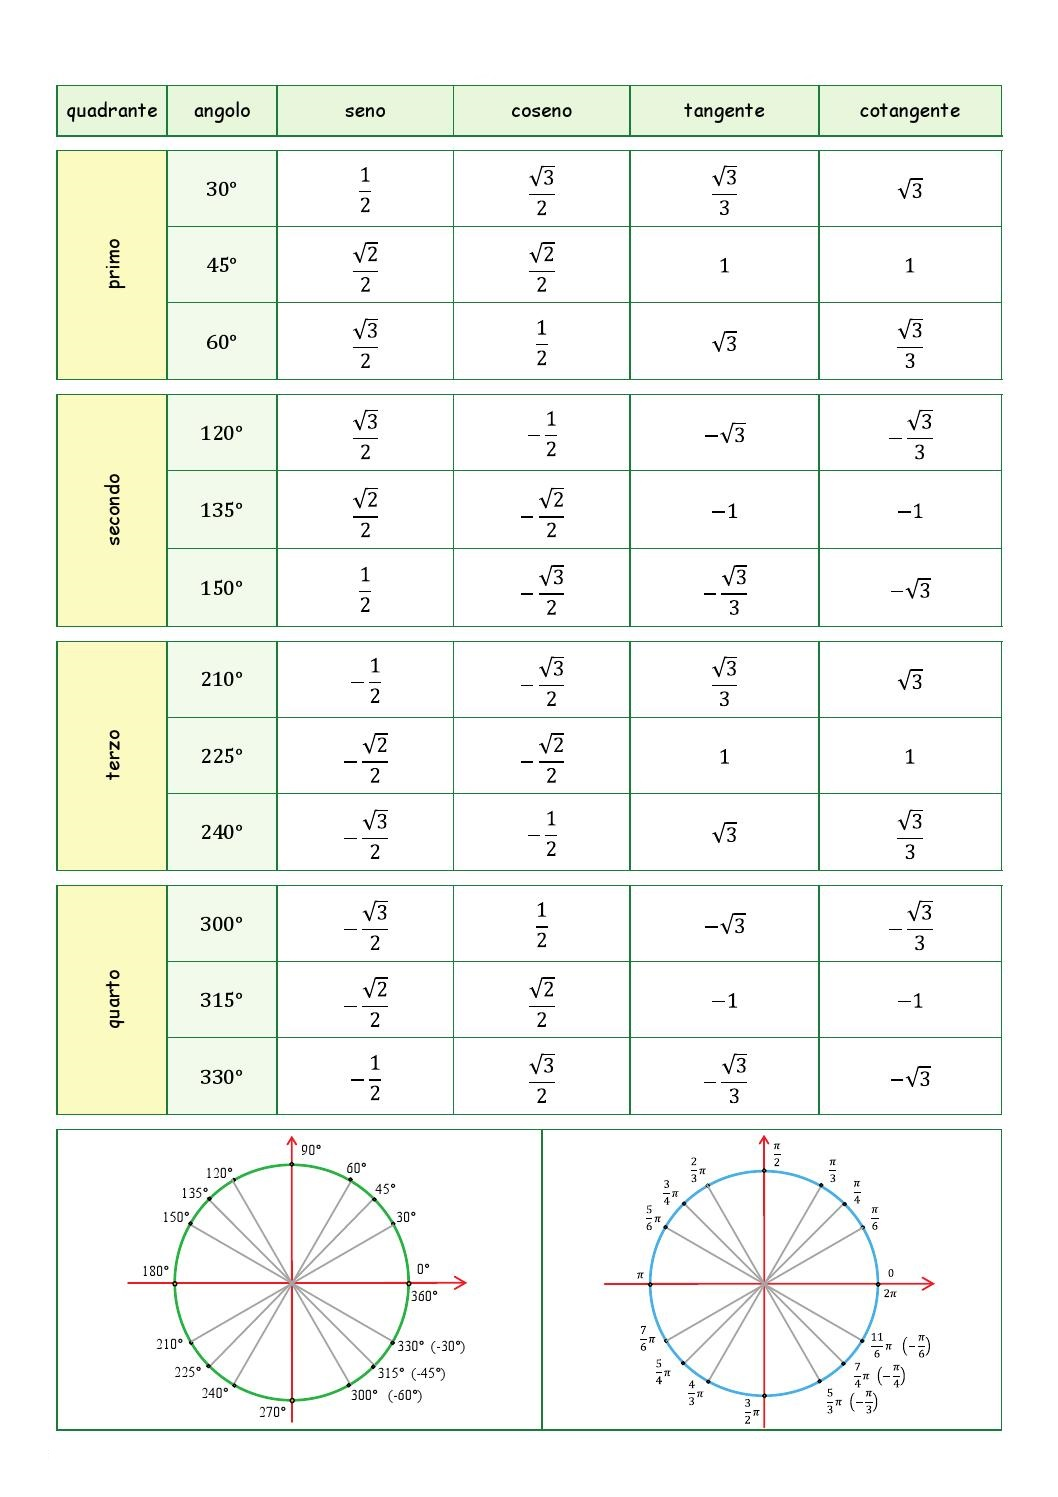
\includegraphics[width=\linewidth]{sincos.jpg}
			\caption{Tabella degli angoli associati}
		\end{figure}
	\end{center}
	
	
	\newpage
	\section{Trigonometria}

	\begin{figure}[htbp]
		\begin{center}
			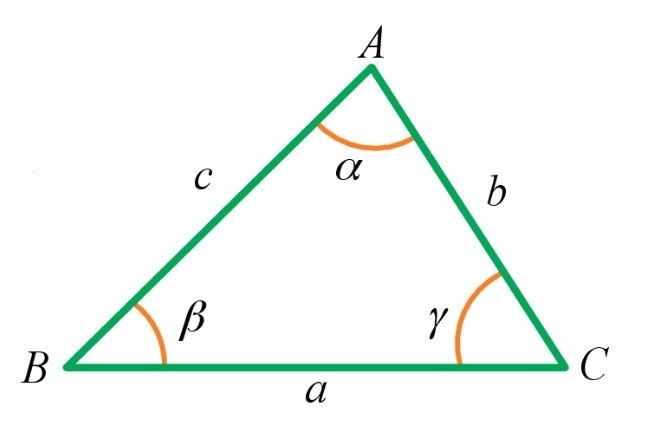
\includegraphics[width=\linewidth]{trigonometria.jpg}
		\end{center}
	\end{figure}



	\subsubsection{Teorema dei seni}
	In ogni triangolo e' costante il rapporto fra ogni lato ed il seno dell'angolo opposto e tale costante equivale al doppio del raggio del cerchio circoscritto al triangolo.
	\begin{align*}
	\frac{a}{\sin \alpha} = \frac{b}{\sin \beta} = \frac{c}{\sin \gamma}\\
	\end{align*}
	
	\subsubsection{Teorema del coseno (Carnot)}
	In ogni triangolo il quadrato di un lato e' uguale alla somma dei quadrati degli altri due lati meno il doppio prodotto degli stessi lati per il coseno dell' angolo fra essi compreso.\\
	\begin{align*}
		a^2 = b^2 + c^2 -2bc\cos \alpha\\
		b^2 = a^2 + c^2 -2ac\cos \beta\\
		c^2 = a^2 + b^2 -2ab\cos \gamma	
	\end{align*}
	
	\newpage
	\section{Esponenziali}
	\begin{align*}
		a^x &= b		&		a>&0
	\end{align*}
		
			\begin{center}
			\begin{tikzpicture}
			\begin{axis}[
			axis lines = left,
			xlabel = $x$,
			ylabel = {$f(x)$},
			xmin=0,xmax=5,
			ymin=0,ymax=10
			]
			
			\addplot [
			domain= 0:6.28,
			samples=100, 
			color=red,
			]
			{e^x};
			\addlegendentry{$e^x$}	
			
					\addplot [
			domain=0:6.28, 
			samples=100, 
			color=blue,
			]
			{ln(x)};
			\addlegendentry{$\ln{x}$}
			\end{axis}
			
			\end{tikzpicture}
		\end{center}
		
	\section{Logaritmi}
	\begin{align*}
		\log_{a}{b} &= x
		&
		\begin{cases}
		b > 0\\
		a > 0 \wedge a \ne 0
		\end{cases}&\\
	\end{align*}
	
	\subsubsection{Proprietà}
	\begin{align*}
		\log_{a}(b \cdot c)                 & = \log_{a} b + \log_{a} c &
		\log_{a} \left( \frac{b}{c} \right) & = \log_{a} b - \log_{a} c \\
		\log_{a} b^n                        & = n \log_{a} b		&
		\log_{a} b 							& = \frac{\log_{c} b}{\log_{c} a}\\
	\end{align*}
	\subsubsection{Casi particolari}
	\begin{align*}
		\\ \log_{a} 1 &= 0 &
		\log_{a} a &= 1
	\end{align*}
		
	\newpage
	\section{Limiti}
	
	\subsubsection{Verifica dei limiti}
	\begin{align*}
		&\forall \epsilon > 0 \exists I(x_0) : \left| f(x) - l \right|<\epsilon	&	\forall &x \in I(x_0),x\ne x_0	&	l,&x_0 \in \mathcal{N}\\\\
		&\forall M > 0 \exists I(x_0) : f(x) - l > M	&	\forall &x \in I(x_0),x\ne x_0	&	l &=+\infty\\\\
		&\forall M > 0 \exists I(x_0) : f(x) - l < -M	&	\forall &x \in I(x_0),x\ne x_0	&	l &=-\infty\\\\
		&\forall \epsilon > 0 \exists c>0: \left| f(x) - l \right| < \epsilon	&	\forall &x>c	&	x_0 &= +\infty\\\\
		&\forall \epsilon > 0 \exists c>0: \left| f(x) - l \right| < \epsilon	&	\forall &x<-c	&	x_0 &= -\infty\\
	\end{align*}
	\subsubsection{Forme indeterminate}
	\begin{align*}
		 & +\infty-\infty &  & 0\cdot \infty &  & \frac{0}{0} &  & \frac{\infty}{\infty} &  & 0^0        \\\\
		 & \infty^0       &  & 1^\infty      &  & \log_{1}1   &  & \log_{0} \infty       &  & \log_{0} 0\\
	\end{align*}
	
	\subsubsection{Limiti notevoli}
	\begin{align*}
		 & \lim\limits_{x \to 0} \left(\frac{\sin x}{x}\right) = 1 &  & \lim\limits_{x \to \pm \infty} \left(1+\frac{1}{x}\right) = 1	&	&\lim\limits_{x \to 0} \left(\frac{1-\cos x}{x^2}\right) = \frac{1}{2}\\\\
		 & \lim\limits_{x \to \infty} (1+x)^{\frac{1}{x}} = e &  & \lim\limits_{x \to 0} \left(\frac{e^x-1}{x}\right) = 1\\
		 \end{align*}
	
	\subsubsection{Teorema del confronto}
	\begin{align*}
	&\begin{cases}
			\mathcal{D}_{f(x)} = \mathcal{D}_{g(x)} = \mathcal{D}_{h(x)}\\
			f(x) \le g(x) \le h(x)
		\end{cases}	&	&\to	&	&\lim f(x) = \lim h(x)	&	&\to	&=\lim g(x)
	\end{align*}
	
	
	\newpage
	\section{Derivate}
	\subsubsection{Derivate immediate}
	\begin{align*}
		&k \in \mathcal{N}  \to 0                       & &x^a          \to	 ax^{a-1}              \\
		&x                  \to 1                       & &\sqrt{x}     \to 	\frac{1}{2\sqrt{x}}   \\
		&\sqrt[n]{x}        \to \frac{1}{n\sqrt[n]{x}}  & &\frac{1}{x}  \to -\frac{1}{x^2}         \\
		&a^x                \to a^x\ln a                & &e^x          \to e^x                    \\
		&\log_{a} x         \to \frac{1}{x} \log_{a} e  & &\ln x        \to \frac{1}{x}            \\
		&\sin x             \to \cos x                  & &\cos x       \to -\sin x                \\
		&\arctan x          \to \frac{1}{1+x^2}         & &\arcsin x    \to \frac{1}{\sqrt{1-x^2}} \\
		&\arccos x          \to -\frac{1}{\sqrt{1-x^2}} &\\
	\end{align*}
	
	\subsubsection{Proprietà}
	\begin{itemize}
		\item Somma:
		\begin{align*}
			d(f(x) + g(x)) = d(f(x))+d(g(x))
		\end{align*}
		\item  Prodotto:
		\begin{align*}
			d(k \cdot f(x)) &= k \cdot d(f(x))\\
			d(f(x) \cdot g(x)) &= f'(x) \cdot g(x) + f(x) \cdot g'(x)
		\end{align*}
		\item Quoziente:
		\begin{align*}
			d\left( \frac{f(x)}{g(x)} \right) = \frac{f'(x) \cdot g(x) - f(x) \cdot g'(x)}{g(x)^2}
		\end{align*}
		\item Reciproco:
		\begin{align*}
			d\left( \frac{1}{f(x)} \right) = -\frac{f'(x)}{f(x)^2}
		\end{align*}
		\item Inverso:
		\begin{align*}
			d \left( f(x)^{-1} \right) = \frac{1}{f'(x)}
		\end{align*}
	\end{itemize}
\newpage
	\subsubsection{Teorema di Rolle}
	Se una funzione è continua in un intervallo chiuso , derivabile in ogni punto dell'intervallo aperto e assume valori uguali negli estremi dell'intervallo, allora esiste almeno un punto interno ad in cui la derivata si annulla, cioè (punto critico o stazionario).
	\\Requisiti:
	\begin{itemize}
		\item $f(x)$ continua e derivabile in $(a;b)$
		\item $f(a) = f(b)$
	\end{itemize}
	\begin{align*}
		\exists c \in \mathcal{N} f'(c) = 0
	\end{align*}
	\subsubsection{Teorema di Cauchy}
	Requisiti:
	\begin{itemize}
		\item $f(x)$ continua e derivabile in $(a;b)$
		\item $g(x)$ continua e derivabile in $(a;b)$
	\end{itemize}
	\begin{align*}
	\frac{f'(c)}{g'(c)} = \frac{f(b)-f(a)}{g(b)-g(a)}
	\end{align*}
	
	\subsubsection{Teorema di Lagrange}
	Dato il grafico di una funzione tra due estremi, esiste almeno un punto in cui la tangente al grafico è parallela alla secante passante per gli estremi.
	Questo teorema è usato per provare delle proprietà di una funzione in un intervallo partendo da ipotesi locali sulle derivate nei punti di tale intervallo.
	Requisiti:
	\begin{itemize}
		\item $f(x)$ continua e derivabile in $(a;b)$
	\end{itemize}
	\begin{align*}
	f'(c)= \frac{f(b)-f(a)}{b-a}
	\end{align*}
	\begin{center}
	\begin{figure}[htpb]
		\begin{minipage}[H]{0.47\textwidth}
			\centering
			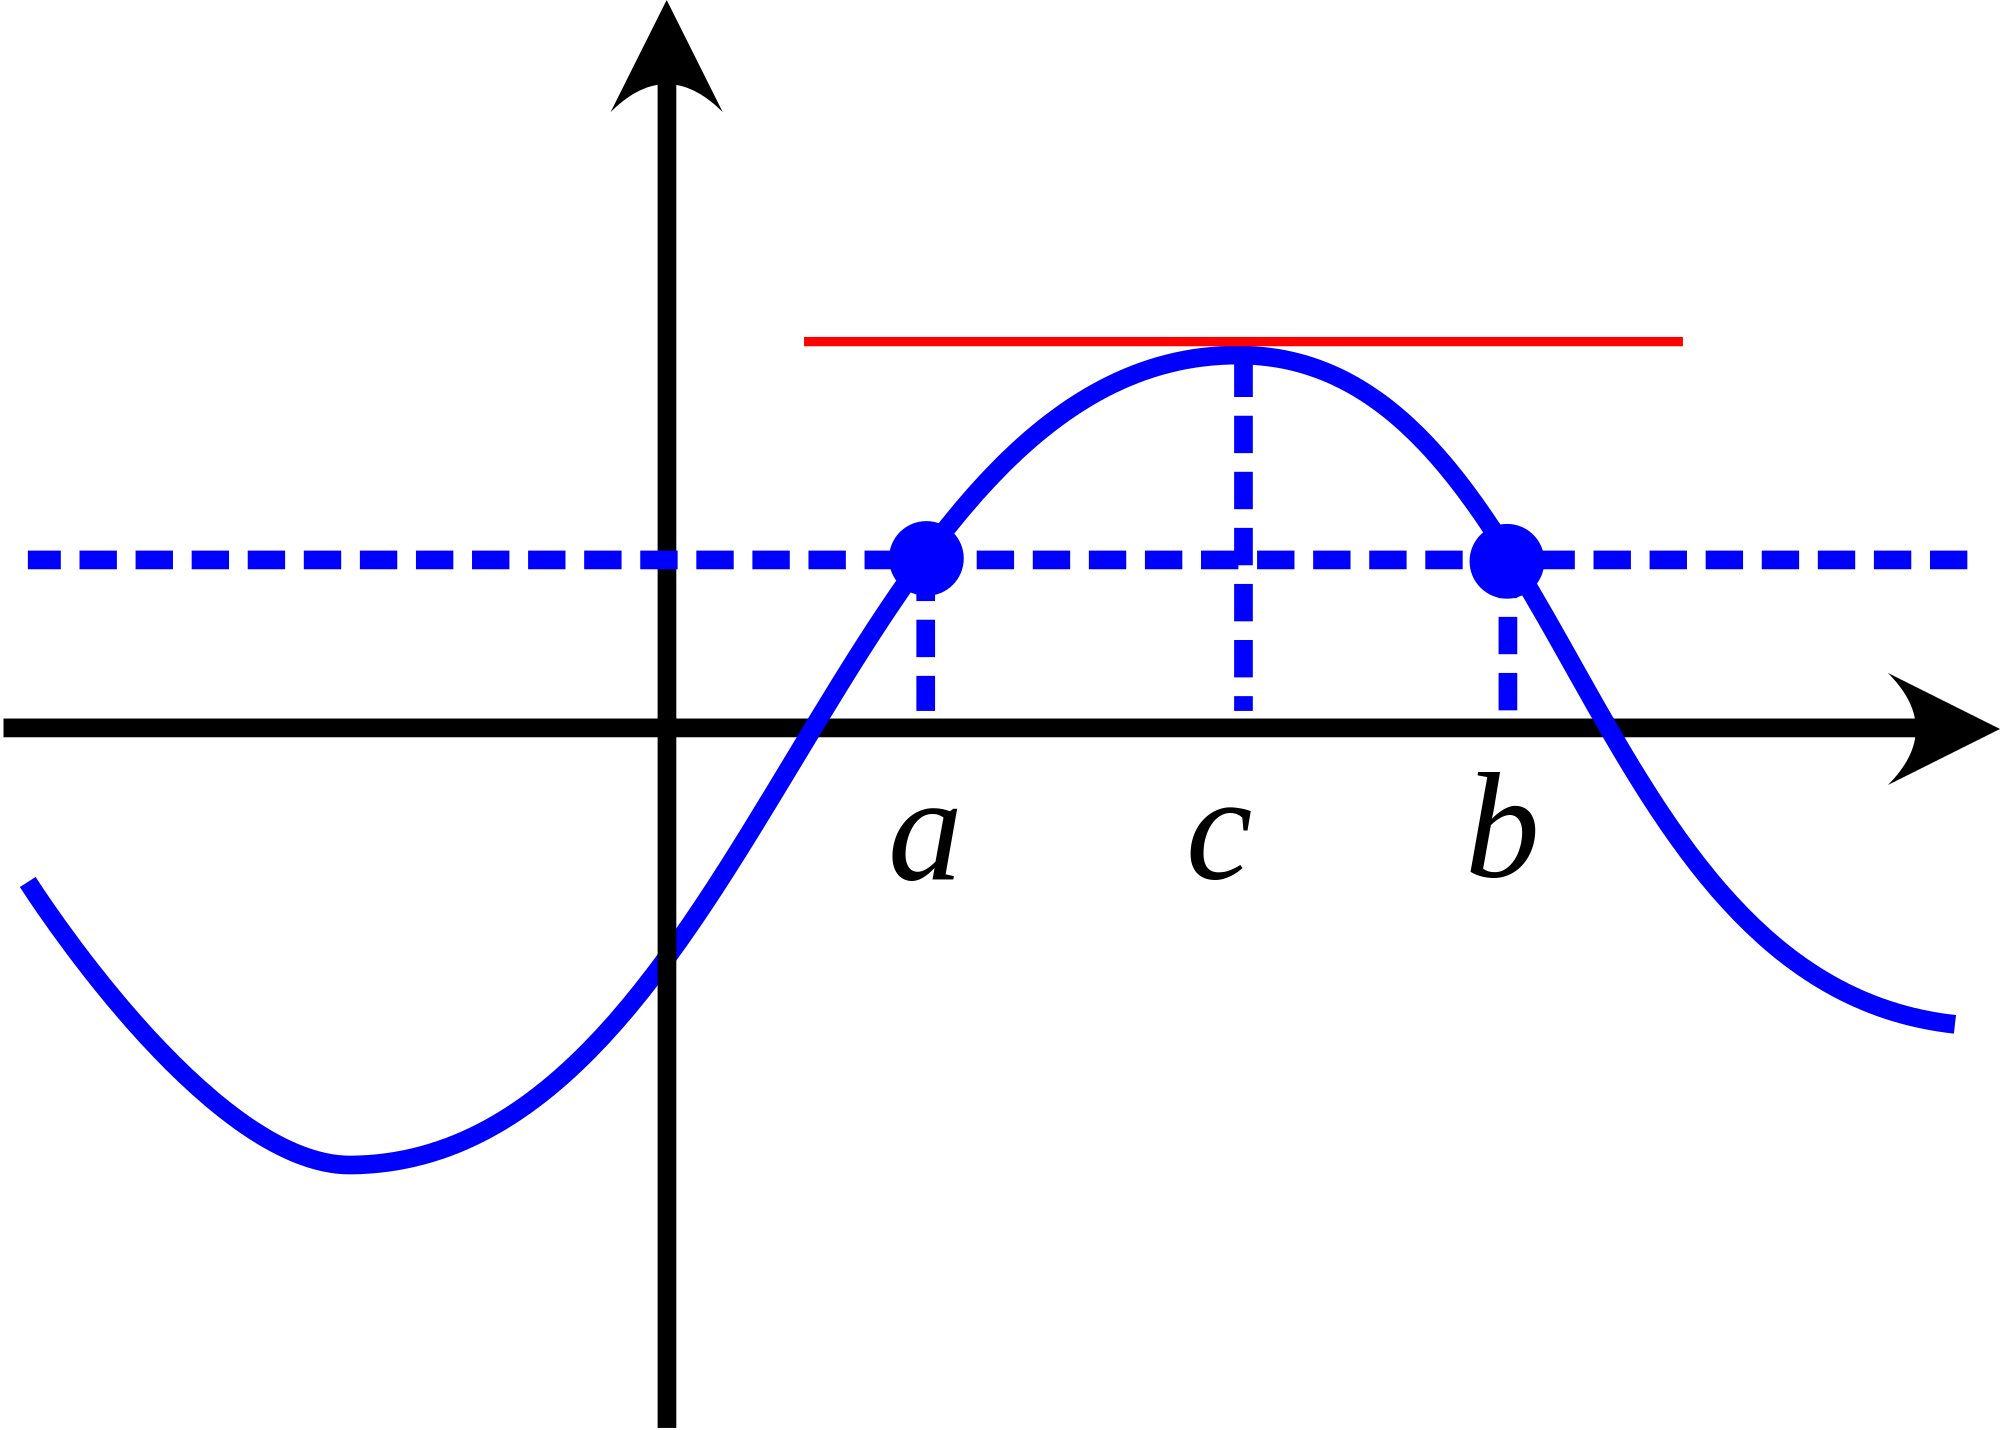
\includegraphics[width=3.7cm]{rolle.png}
			\caption{\label{f_etichetta1}Teorema di Rolle}
		\end{minipage}
		\hfill
		\begin{minipage}[H]{0.47\textwidth}
			\centering
			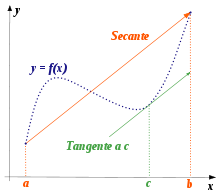
\includegraphics[width=3.7cm]{lagrange.png}
			\caption{\label{f_etichetta1}Teorema di Lagrange}
		\end{minipage}
	\end{figure}
		
	\end{center}
	
	\newpage
	\subsection{Teorema delle derivate successive}
	Massimo:\\
	\begin{align*}
		\begin{cases}
			f'(x_0) = 0\\
			f''(x_0) < 0
		\end{cases}
	\end{align*}
	Minimo:\\
	\begin{align*}
		\begin{cases}
			f'(x_0) = 0\\
			f''(x_0) > 0
		\end{cases}
	\end{align*}
	Flesso ascendente a tangente orizzontale:\\
	\begin{align*}
		\begin{cases}
			f'(x_0) = 0\\
			f''(x_0) = 0\\
			f'''(x_0) > 0
		\end{cases}
	\end{align*}
	Flesso discendente a tangente orizzontale:\\
	\begin{align*}
		\begin{cases}
			f'(x_0) = 0\\
			f''(x_0) = 0\\
			f'''(x_0) < 0
		\end{cases}
	\end{align*}	
	Flesso ascendente a tangente obliqua:\\
	\begin{align*}
	\begin{cases}
	f'(x_0) \ne 0\\
	f''(x_0) = 0\\
	f'''(x_0) > 0
	\end{cases}
	\end{align*}	
	Flesso discendente a tangente obliqua:\\
	\begin{align*}
	\begin{cases}
	f'(x_0) \ne 0\\
	f''(x_0) = 0\\
	f'''(x_0) < 0
	\end{cases}
	\end{align*}	
	Formula della tangente obliqua:
	\begin{align*}
		y-y_0 = f'(x_0)(x-x_0)
	\end{align*}
	
	
	
	
	\newpage
	\section{Integrali}
	\subsubsection{Proprietà}
	\begin{align*}
		\int k f(x) dx &= k \int f(x) dx\\
		\int \left[f_1(x)+f_2(x)+f_3(x)\right]dx &= \int f_1(x)dx + \int f_2(x)dx + \int f_3(x)dx\\
	\end{align*}
	
	\subsubsection{Integrali immediati}
	\begin{align*}
		&\int x^\alpha dx             = \frac{x^{\alpha + 1}}{\alpha + 1} +c & &\int \frac{1}{x}dx      = \ln|x| + c              &  &\int \sin (x) dx               = -\cos(x) + c    \\
		                            &                                        &  \\
		&\int \cos (x) dx             = \sin (x) +c                          & &\int \frac{1}{1+x^2}dx  = \arctan (x) +c          & &\int \frac{1}{\cos^2 (x)}dx    = \tan (x) + c    \\
		                            &                                        &  \\
		&\int e^x dx                  = e^x +c                               & &\int a^x dx             = \frac{a^x}{\ln (a)} + c & &\int \frac{1}{\sqrt{a-x^2}}dx  = \arcsin (x) + c \\
		                            &  \\
		&\int \frac{1}{\sin^2 (x)}dx  = -\cot(x) + c                         & &\int 1 dx               = x+c                     &\\
	\end{align*}
	
	\subsubsection{Integrali mediati}
	\begin{align*}
		&\int [f(x)]^\alpha \cdot f'(x) dx 	= \frac{[f(x)]^{\alpha + 1}}{\alpha + 1}+c		&	&\int \frac{f'(x)}{f(x)}dx = \ln |f(x)| + c\\\\
		&\int f'(x) \cdot \sin [f(x)] dx		= -\cos [f(x)] + c								&	&\int f'(x) \cdot \cos [f(x)] dx = \sin [f(x)] + c\\\\
		&\int e^{f(x)} \cdot f'(x) dx 		= e^{f(x)}+c									&	&\int \frac{f'(x)}{\sqrt{1-f^2(x)}}dx = \arcsin[f(x)] + c\\\\
		&\int a^{f(x)} \cdot f'(x) dx		= \frac{a^{f(x)}}{\ln (a)}+c					&	&\int \frac{f'(x)}{1+f^2(x)}dx = \arctan [f(x)] + c\\\\
		&\int \frac{f'(x)}{\cos^2 [f(x)]}dx	= \tan [f(x)] + c  		
	\end{align*}
	\subsubsection{Funzioni non banali}
	Risoluzione con formule parametriche:
	\begin{align*}
		\sin (x) &= \frac{2t}{1+t^2}		&		\cos (x) &= \frac{1-t^2}{1+t^2}			& 	t &= \tan \left( \frac{x}{2} \right)
	\end{align*}
	Risoluzione di integrali irrazionali:
	\begin{align*}
		\int & \sqrt{x^2 \pm \alpha^2}	dx		&		\int  \frac{1}{\sqrt{x^2 \pm \alpha^2}}dx&	&	\rightarrow t &= x + \sqrt{x^2 \pm \alpha^2}\\\\
		\int \sqrt{a^2 - x^2}dx &= \frac{a^2}{2}\arcsin \left( \frac{x}{a} \right) + \frac{x}{2}\sqrt{a^2-x^2}	&&	&		\rightarrow x &= a\sin (t)
	\end{align*}
	Risoluzione per parti:
	\begin{align*}
		\int f(x) \cdot g'(x) dx = f(x) \cdot g(x) - \int f'(x) \cdot g(x) dx
	\end{align*}
		
	\subsubsection{Teorema della media}
	\begin{align*}
		f(c) = \frac{\int_{a}^{b}f(x)dx}{b-a}
	\end{align*}
	\subsubsection{Volume nei solidi di rotazione}
	\begin{align*}
		V =\pi \int_{a}^{b} f^2(x)dx
	\end{align*}
	
	\subsubsection{Metodo dei rettangoli}
	\begin{align*}
		\int_{a}^{b}f(x)dx &= \frac{b-a}{n}\sum_{i=0}^{n-1}f(x_i)		&\vee&	&	\int_{a}^{b} f(x)dx =\frac{b-a}{n}\sum_{i=0}^{n} f(x_i)		
	\end{align*}
	
	\subsubsection{Metodo dei trapezi}
	\begin{align*}
		\frac{b-a}{n}\sum_{i=0}^{n-1}\frac{f(x_i)+f(x_i + 1)}{2} = \int_{a}^{b} f(x)dx
	\end{align*}
	
	
	\newpage
	\subsubsection{Integrali doppi}
	\begin{align*}
		I = \int_{a}^{b}dy\int_{c}^{d}f(x,y)dx
	\end{align*}
	\subsubsection{Integrali di linea di prima specie}
	\begin{align*}
		I = \int_{a}^{b}f(\gamma (t)) \cdot ||\gamma'(t)||dt
	\end{align*}
	
	\subsubsection{Integrali di linea di seconda specie}
		\begin{align*}
		\gamma:&[a,b] \to \mathcal{R}^2	&	\vec{F}:&(x,y)\to(x_1,y_1)	&	t &\to (t_1,t_2)
		\end{align*}
		\begin{align*}
			\int_{a}^{b}<(f(\gamma));(\gamma'(t))> dt
		\end{align*}
	\subsubsection{Integrali tripli}
	\begin{itemize}
		\item Parallelepipedi regolari:
		\begin{align*}
			D = [a,b] \times [c,d] \times [e,h] \to \int_{a}^{b}\left( \int_{c}^{d} \left( \int_{e}^{h} f(x,y,z) dz \right) dy \right) dx
		\end{align*}		
		\item Per fili:
		\begin{align*}
			D = \left\lbrace  (x,y,z) \in \mathcal{R}^2:(x,y) \in \Omega,g_1(x,y) \le z \le g_2(x,y) \right\rbrace to \int \int_{\Omega} \left( \int_{g_1(x,y)}^{g_2(x,y)}f(x,y,z)dz \right)dxdy
		\end{align*}
		\item Per strati:
		\begin{align*}
		D =	\left\lbrace (x,y,z) \in \mathcal{R}^2:z_1 \le z \le z_2 , (x,y) \in \Omega (z) \right\rbrace \to \int_{z_1}^{z_2} \left( \int \int_{\Omega (z)} f(x,y,z)dxdy \right)dz
		\end{align*}
	\end{itemize}
	\subsubsection{Campi vettoriali}
	\begin{enumerate}
		\item Verificare che il campo sia conservativo con le derivate incrociate:
		\begin{align*}
			F'_{ij} = F'_{ji}
		\end{align*}
		\item Trovare il potenziale (U è il minimo potenziale che comprende entrambi gli integrali):
		\begin{align*}
			&\vec{F}:(x,y) \to (x_1,y_2)	&	&\begin{cases}
			\int x_1 dx\\
			\int y_1 dy
			\end{cases}	&	&\int_{a}^{b}\vec{F} = U(\gamma)_B - U(\gamma)_B
		\end{align*}
	\end{enumerate}
	
	\newpage
	\section{Equazioni differenziali}
	\subsubsection{Primo ordine}
	\begin{align*}
			F(y';y;x)=0
	\end{align*}
	\begin{enumerate}
		\item $y' = f(x)$
		\begin{align*}
			\frac{dy}{dx}&=f(x)		&		y &= \int f(x)dx
		\end{align*}
		\item $y'=g(x)\cdot h(x)$ con $h(y) \ne 0$
		\begin{align*}
			\frac{dy}{dx} &= g(x)h(y)	&	\frac{dy}{h(y)} &= g(x)dx	&	\int \frac{dy}{h(y)}=\int g(x)dx
		\end{align*}
		\item $y'+a(x)y = b(x)$
		\begin{align*}
			y = e^{-\int a(x)dx}\cdot \left[ \int b(x)\cdot e^{\int a(x)dx} dx + c \right]
		\end{align*}
	\end{enumerate}
	\subsubsection{Secondo ordine}
	\begin{enumerate}
		\item $F(y'';y';y;x)=0$
		\begin{align*}
			y'' + by' + cx = 0 &\to z^2+bz+c=0		&		&\begin{cases}
			y = c_1e^{z_1x}+c_2e^{z_2x}		&	\varDelta > 0\\
			y = e^{zx}(c_1+c_2x)	&	\varDelta =0\\
			y = e^{\alpha x}(c_1\cos{\beta x} + c_2\sin{\beta x})	&	\varDelta<0
			\end{cases}
		\end{align*}
		\item $y'' +by' + cy = r(x)$\\\\
		Risolvere la soluzione omogenea $y'' +by' + cy = 0$ e poi valutare la soluzione particolare $r(x)$:
		\begin{itemize}
			\item  $r(x)$ polinomio $\to p(x) = x(ax^2+bx+c) $ \\
			\item  $r(x) = A \cdot e^{hx} \to p(x) = C \cdot e^{rx}$ , $r=h$\\
			\item  $r(x) = A \cos{\omega x} + B\sin{\omega x} \to p(x) = C\cos{\omega x} + D\sin{\omega x}$
		\end{itemize}
	\end{enumerate}
	
	
	
	\newpage
	\section{Studio di funzione}
		\subsection{Studio del dominio}
		Verificare la presenza di:\\
		\begin{align*}
			&\frac{numeratore}{denominatore} & &\to & &denominatore \ne 0\\\\
			&\sqrt{argomento}				 & &\to & &argomento \ge 0\\\\
			&\log_{a}{(argomento)}			 & &\to & &argomento > 0\\
		\end{align*}
		
		\subsection{Studio del limite e degli asintoti}
		\subsubsection{Discontinuità}
		\begin{itemize}
			\item  Funzione continua:
			\begin{align*}
			\lim\limits_{x \to x_0^-} f(x) = \lim\limits_{x \to x_0^+} f(x)
			\end{align*}
			\item  Discontinuità di prima specie:
			\begin{align*}
			\lim\limits_{x \to x_0^-} f(x) \ne \lim\limits_{x \to x_0^+} f(x) \in \mathcal{R}
			\end{align*}
			\item  Discontinuità di seconda specie:
			\begin{align*}
			\lim\limits_{x \to x_0^-} f(x) \ne \lim\limits_{x \to x_0^+} f(x) = \pm \infty
			\end{align*}
			\item Discontinuità di terza specie:
			\begin{align*}
			\lim\limits_{x \to x_0^-} f(x) = \lim\limits_{x \to x_0^+} f(x) \wedge x \ne x_0
			\end{align*}
			
		\end{itemize}
		
		\subsubsection{Asintoto}
		\begin{itemize}
			\item Orizzontale\\
			\begin{align*}
				&\lim\limits_{x \to \pm \infty}{f(x)} = q	&	y&=q
			\end{align*}
			
			\item Verticale\\
			\begin{align*}
				&\lim\limits_{x \to q}{f(x)} = \pm \infty	&	x&=q
			\end{align*}
			\item Obliquo\\
			\begin{align*}
			&\lim\limits_{x \to \pm \infty}{f(x)} = \pm \infty	&	y&=mx+q\\
			&m=\lim\limits_{x \to \pm \infty}{\frac{f(x)}{x}}   &	q&=\lim\limits_{x \to \pm \infty}{f(x)-mx}
			\end{align*}
						
		\end{itemize}
		
		\subsection{Parità/Disparità}
		\begin{itemize}
			\item \textbf{Funzione pari:} funzione simmetrica rispetto all'asse y.
			\begin{align*}
				f(x) &= f(-x)
			\end{align*}
			\item \textbf{Funzione dispari:} funzione con simmetria centrale rispetto all'origine.
			\begin{align*}
				f(x) &= -f(-x)
			\end{align*}
		\end{itemize}
		
		\subsection{Incontro con gli assi}
		\begin{align*}
			&\begin{cases}
			x = 0\\
			y = f(0)
			\end{cases}	&	&\bigcup &	&\begin{cases}
			y = 0\\
			f(x) = 0
			\end{cases}
		\end{align*}
		
		\subsection{Studio del segno}
		\begin{align*}
			f(x) > 0
		\end{align*}
		Funzione crescente:
		\begin{align*}
			\forall x_1,x_2 \in \mathcal{D}, x_1 < x_2 &\to f(x_1)<f(x_2)
		\end{align*}
		Funzione decrescente:
		\begin{align*}
			\forall x_1,x_2 \in \mathcal{D}, x_1 > x_2 &\to f(x_1)>f(x_2)
		\end{align*}

		\subsection{Punti di massimo e minimo}
		Line up:
		\begin{enumerate}
			\item Calcolo della derivata prima
			\item Studio del dominio
			\item Studio del segno
			\begin{align*}
				f'(x) > 0
			\end{align*}
			\item Estrazione del massimo e minimo locale/globale 
		\end{enumerate}
		
		
		\subsection{Punti di flesso}
		Line up:
		\begin{enumerate}
			\item Calcolo della derivata seconda
			\item Studio del dominio
			\item Studio del segno
			\begin{align*}
			f''(x) > 0
			\end{align*}
			\item Estrazione del massimo e minimo locale/globale 
		\end{enumerate}		
	\newpage
	\subsection{Punti di non derivabilità}
	Punto angoloso:
	\begin{align*}
		\lim\limits_{x \to x_0^-}f'(x) \ne \lim\limits_{x \to x_0^+}f'(x)
	\end{align*}
	Cuspide:
	\begin{align*}
		\lim\limits_{x \to x_0^-}f'(x) \ne \lim\limits_{x \to x_0^+}f'(x) = \pm \infty
	\end{align*}
	Flesso a tangente verticale:
	\begin{align*}
		\lim\limits_{x \to x_0^-}f'(x) = \lim\limits_{x \to x_0^+}f'(x) = \pm \infty
	\end{align*}
	
	\subsection{Proprietà delle funzioni derivabili}
	\begin{center}
		\begin{tabular}{|c|c|}
		\hline 
		\textbf{f(x)} & \textbf{f'(x)} \\ 
		\hline 
		$x \ne k$ & $x \ne k$ \\ 
		\hline 
		$pari$ & $dispari$ \\ 
		\hline 
		$dispari$ & $pari$ \\ 
		\hline 
		$crescente$ & $positiva$ \\ 
		\hline 
		$decrescente$ & $negativa$ \\ 
		\hline 
		$max/min$ & $intersezione$ \\ 
		\hline
		$\cap$	&	$decrescente$ \\
		\hline
		$\cup$	&	$crescente$	\\
		\hline
		$flesso$ & $max/min$	\\
		\hline
		\end{tabular} 
	\end{center}
	
	\subsection{Approssimazioni}
	\subsubsection{Metodo delle tangenti (Newton)}
	Il metodo delle tangenti, chiamato anche metodo di Newton-Raphson, è uno dei metodi per il calcolo approssimato di una soluzione di un'equazione della forma $f(x)=0$. Esso si applica dopo avere determinato un intervallo $[a,b]$ che contiene una sola radice.
	
	\begin{align*}
		C_n = C_{n-1}-\frac{f(n-1)}{f'(n-1)}
	\end{align*}
	\subsubsection{Metodo delle secanti}
	Il metodo delle secanti è uno dei metodi più semplici per il calcolo approssimato di una soluzione di un'equazione della forma $f(x)=0$. Esso si applica dopo avere determinato un intervallo $[a,b]$ che contiene una sola radice.
	\begin{align*}
		C_{n+1} = b-\frac{f(b)\cdot (b-C_n)}{f(b)-f(C_n)}
	\end{align*}
	
	
	
	
	
	
	
	
	
	
	
	
	
	
	
	
	
	
	
	
	
	
	
	
	
	
	
	
	
	
	
	
	
	
	
	
	
	
	
	
	
	
	
	
	
	
	
	
	
	
	
	
\end{document}